% "{'classe':('PSI'),'chapitre':'chs_leq','type':('cours'),'titre':'Détermination des liaisons équivalentes', 'source':'','comp':('B2-12','B2-15'),'corrige':True}"
\setchapterimage{Fond_CIN.png}
\setchapterpreamble[u]{\margintoc}

\chapter{Détermination des liaisons équivalentes}

\marginnote[2cm]{
\UPSTIcompetence[2]{B2-12}
\UPSTIcompetence[2]{B2-15}
}


%\marginnote[]{}

\begin{marginfigure}[4cm]
\centering
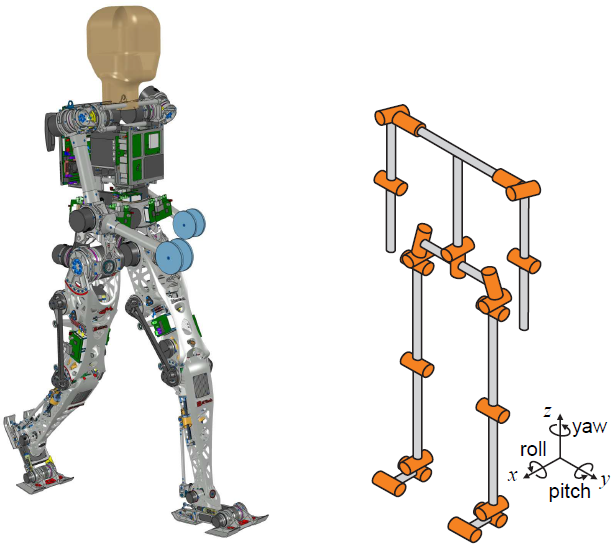
\includegraphics[width=0.6\textwidth]{lola}
\caption{Robot humanoïde Lola}
\end{marginfigure}

\begin{marginfigure}[8cm]
\centering
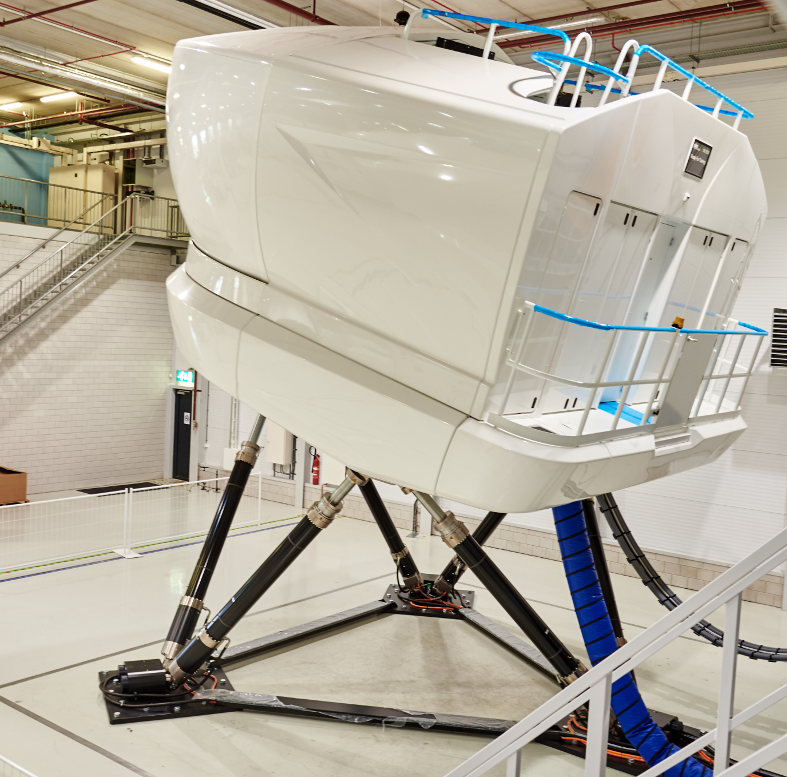
\includegraphics[width=0.5\textwidth]{simu}
\caption{Simulateur de vol Lockheed Martin}
\end{marginfigure}



\section{Introduction}
\subsection{Rappel sur les torseurs des liaisons}
\begin{defi}[Torseur cinématique]
De manière générale, le torseur cinématique peut être noté :
$$
\torseurcin{V}{i}{j}
=\torseurl{\vecto{i}{j}}{\vectv{P}{i}{j}}{P}
=\torseurl{p_{ij}\vect{x}+q_{ij}\vect{y}+r_{ij}\vect{z}}{u_{ij}\vect{x}+v_{ij}\vect{y}+w_{ij}\vect{z}}{P}
=\torseurcol{p_{ij}}{q_{ij}}{r_{ij}}{u_{ij}}{v_{ij}}{w_{ij}}{P,\mathcal{R}}.
$$

\textbf{On notera $n_c$ le nombre d'inconnues cinématiques d'une liaison.} En d'autres termes, $n_c$ correspond donc au nombre de mobilités de la liaison.
\end{defi}

\begin{defi}[Torseur Statique]
De manière générale, le torseur statique peut être noté :
$$
\torseurstat{T}{i}{j}
=\torseurl{\vectf{i}{j}}{\vectm{P}{i}{j}}{P}
=\torseurl{X_{ij}\vect{x}+Y_{ij}\vect{y}+Z_{ij}\vect{z}}{L_{ij}\vect{x}+M_{ij}\vect{y}+N_{ij}\vect{z}}{P}
=\torseurcol{X_{ij}}{Y_{ij}}{Z_{ij}}{L_{ij}}{M_{ij}}{N_{ij}}{P,\mathcal{R}}.
$$

\textbf{On notera $n_s$ le nombre d'inconnues statiques d'une liaison.} En d'autres termes, $n_s$ correspond au degré de liaison. On a $n_s=6-n_c$.
\end{defi}
\subsection{Graphe des liaisons}

\begin{defi}[Chaînes et cycles]
Selon la forme du graphe de liaisons, on peut distinguer 3 cas :
\begin{multicols}{3}
\begin{center}
\textbf{Les chaînes ouvertes} 
\end{center}

\begin{center}
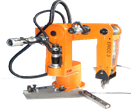
\includegraphics[width=.6\linewidth]{ericc_01}

\vspace{.5cm}

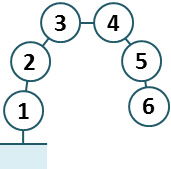
\includegraphics[width=.6\linewidth]{ericc_02}
\end{center}

\vspace{.5cm}

\begin{center}
\textbf{Les chaînes fermées} 
\end{center}

\begin{center}
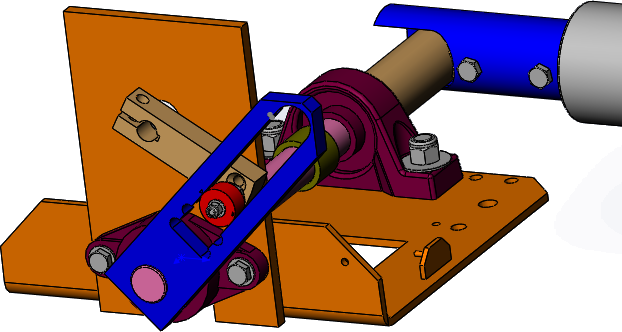
\includegraphics[width=.8\linewidth]{sympact_01}

\vspace{.5cm}

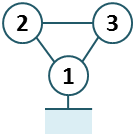
\includegraphics[width=.6\linewidth]{sympact_02}
\end{center}

\vfill\null
\columnbreak

\begin{center}
\textbf{Les chaînes complexes} 
\end{center}

\begin{center}

\includegraphics[width=.95\linewidth]{haptique_01}

\vspace{.5cm}

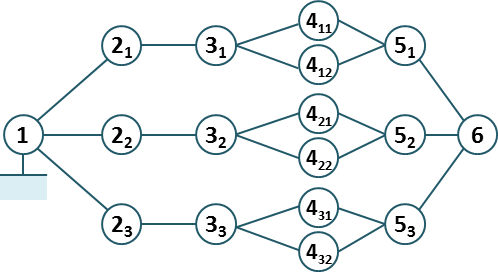
\includegraphics[width=.95\linewidth]{haptique_02}
\end{center}

\end{multicols}

On appelle cycle, un chemin fermé ne passant pas deux fois par le même sommet.
À partir d’un graphe des liaisons donné, il est possible de vérifier qu’il existe un nombre
maximal de cycles indépendants. Ce nombre est appelé nombre cyclomatique. 

\textbf{En notant $L$ le nombre de liaisons et $S$ le nombre de solides, on note $\gamma$ le nombre cyclomatique et on a : $\gamma = L - S + 1$.}
\end{defi}

\begin{remarque}[s]
\begin{itemize}
\item Dans le cas d'une chaîne ouverte, $\gamma$ est nul. 
\item Le degré d'hyperstatisme d'une chaîne fermée << simple >> ne peut pas excéder~6.
\item À partir du graphe de structure, il est possible de déterminer le nombre cyclomatique d'une chaîne complexe... si elle n'est pas trop complexe.

\end{itemize}
\end{remarque}

\section{Liaisons équivalentes}
\begin{obj}
La détermination de la liaison équivalente correspondant à l'association de plusieurs liaisons doit permettre : 
\begin{itemize}
\item de transmettre les mêmes actions mécaniques que l'association de liaisons;
\item d'autoriser les mêmes mouvements relatifs que l'association de liaisons.
\end{itemize}
\end{obj}

\subsection{Liaisons en parallèles}
\begin{methode}
La liaison équivalente aux liaisons en parallèles doit permettre de transmettre la somme de chacune des actions mécaniques. Ainsi : 
$$
\torseurstat{T}{1}{2}_{\text{eq}} = \sum\limits_{i=1}^{n}\torseurstat{T}{1}{2}_{i}.
$$ 
\end{methode}

\begin{remarque}
La liaison équivalente devant permettre les même mobilités que les liaisons en série, il est donc aussi possible de déterminer la liaison équivalente en résolvant le système d'équation suivant : 
$$
\torseurcin{V}{1}{2}_{\text{eq}} 
= \torseurcin{V}{1}{2}_1
= \torseurcin{V}{1}{2}_2
=...
= \torseurcin{V}{1}{2}_n.
$$ 
Cependant cette méthode dite << cinématique >> est moins aisée à mettre en \oe{}uvre que la première.

\end{remarque}
\subsection{Liaisons en série}
\begin{methode}
La liaison équivalente aux liaisons en série se détermine en utilisant la composition du torseur cinématique. En effet : 
$$
\torseurcin{V}{1}{n}_{\text{eq}} = \sum\limits_{i=1}^{n-1}\torseurcin{V}{i}{i+1}.
$$ 
\end{methode}

\begin{remarque}
L'application successive du principe fondamental de la statique à chacun des solides permet de déterminer le torseur équivalent de la liaison : 
$$
\torseurstat{T}{n}{1}_{\text{eq}} = 
\torseurstat{T}{2}{1} = 
\torseurstat{T}{3}{2} =
...
=\torseurstat{T}{n}{n-1}.
$$ 
\end{remarque}

\begin{warn}
L'observation de la forme du torseur de la liaison équivalente ne suffit pas à déduire le nom de la liaison : il faut aussi s'assurer que les composantes du torseur sont bien indépendantes. 
\end{warn}

\subsection{Décomposition des liaisons}
Chacune des liaisons normalisées à $n$ degré de liberté peut être décomposée en $n$ liaisons ponctuelles en parallèles (sphère -- plan). Par exemple, une liaison rotule (sphérique) est équivalente à 3 liaisons ponctuelles en parallèles dont les normales sont non coplanaires et concourantes en un point.